\pagebreak
\section{Vehicle Tests}
\nopagebreak

\subsection{Inertia Test} %\label{put a label here and uncomment}
\textbf{Name: Group 510}\\
\textbf{Date: 02/11 - 2015}

\subsubsection{Purpose}
The purpose of the test is to measure the inertia of the vehicle, $J_{tot}$, and find the vehicle's step-response at the same time.

\subsubsection{Theory}
%-- Not the right test anymore, but could still be useful in case we change our minds --%
% The \figref{inertiaTestPowerCutOrDisable} shows the vehicle's velocity variations throughout time, both when the motor is unplugged manually or when its power is cut via software :

% \begin{figure}[H]
%   \centering
%   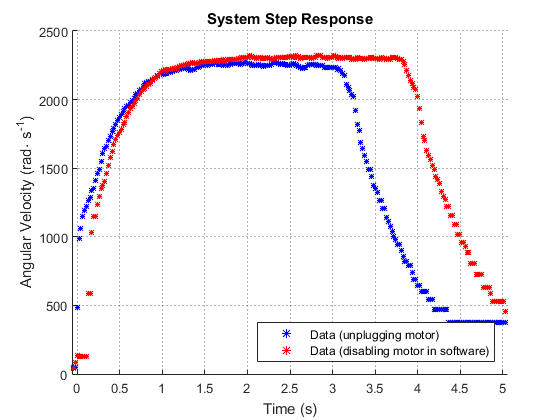
\includegraphics[scale=0.8]{figures/inertiaTestPowerCutOrDisable.png}
%   \caption{Plot of the systems step-response, which is angular velocity over time. The blue dots represents the measured data when the plus-pole of the motor is unplugged manually to stop the vehicle. The red dots represents the measured data when the software is used to stop the vehicle.}
%   \label{inertiaTestPowerCutOrDisable}
% \end{figure}

% By comparing both methods to cut off the motor's power, the back electromotive force generated by the motor when using the software method seems negligible since both curves have very similar decreasing shapes. Moreover, the manual unplugging of the powering wires brings some uncertainty due to a potential disturbance of the force applied to the vehicle.\\
% Therefore, the software method is used to extract the inertia.
%-- End of the first test version --%

In this test a two-step input is used to get the system's response. The reason for this is to avoid the stiction (also called Coulomb friction) when the vehicle starts. The second step input is not sent until the vehicle is in a steady and non-zero velocity. Without these two steps the first data points of the response are unusable, as seen on \figref{MomentOfInertiaTestPlot}.


\subsubsection{Setup}
\begin{figure}[H]
	\centering
	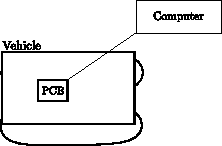
\includegraphics[scale=1.6]{figures/inertiaTestSetupDiagram2.pdf}
	\caption{Setup diagram}
	\label{inertiaTestSetupDiagram}
\end{figure}

\subsubsection{List of Equipment}

\begin{table}[H]
\begin{tabular}{|p{10cm}|p{4cm}|}
\hline%------------------------------------------------------------------------------------
  \textbf{Instrument}                     &  \textbf{Type}       \\
\hline%------------------------------------------------------------------------------------
  Computer                                &  Asus N73JN    \\
\hline %-----------------------------------------------------------------------------------
\end{tabular}
\end{table}

\subsubsection{Procedure}

\begin{enumerate}
  \item Disconnect the battery.
  \item Connect the Arduino to the computer.
  \item Upload the test code to the Arduino board using the Arduino IDE  \cite{ArduinoIDE}.
  \item Open a serial terminal via PuTTY \cite{PuTTY}.
  \item Plug in the battery immediately after opening the terminal.
  \item Wait two seconds, then follow the vehicle with the connected computer.
  \item Wait until the vehicle stops before ending the measurements by unplugging the connected computer from the Arduino.
  \item Plot the speed of the vehicle using Matlab.
\end{enumerate}

\subsubsection{Results} \label{inertiaTestResults}
The execution of the test has a duration of 10 seconds in total. First the vehicle waits for 2 seconds without moving. Thereafter it moves with a 20 percent of its maximal velocity in a duration of 3 seconds. In the last 5 seconds of the test, the vehicle runs at its maximal velocity. These velocity variations in the test can be seen in \figref{MomentOfInertiaTestPlot}.

\begin{figure}[H]
  \centering
  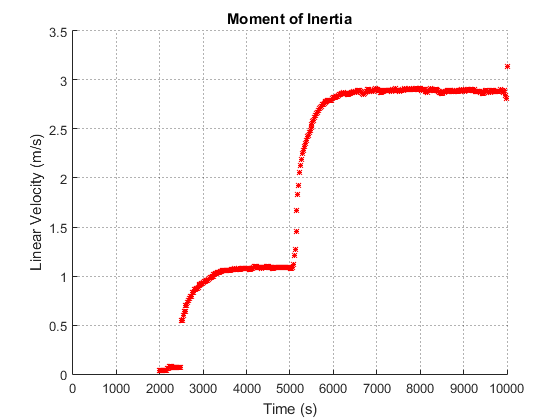
\includegraphics[scale=0.8]{figures/VehicleMomentOfInertiaTest.png}
  \caption{Vehicle's velocity response to a two-steps input}
  \label{MomentOfInertiaTestPlot}
\end{figure}

% \paragraph{Step Response Time Constant}
By knowing the maximum velocity of the vehicle at the end of the test and the velocity when it is in a first steady state, just before the second step, it is possible to deduce the time at which the velocity reaches \si{\num{63.2} \%} of its final value. The obtained time is the step response time constant of the system $\tau$.

Since the velocity is taken at \si{\num{63.2} \%} between the first steady state and the final value, it is needed to shift it up with the starting value $V_{ss1}$ :
\begin{flalign}
\eq{V(\tau)}{(V_{max} - V_{ss1}) \cdot 0.632 + V_{ss1}} \unit{m \cdot s^{-1}}
\end{flalign}
\hspace{6mm} Where:\\
\begin{tabular}{p{1cm}lll}
& $V(\tau)$ & is the velocity of the vehicle at \si{\num{63.2} \%} between the first step and its final value &\unitWh{m \cdot s^{-1}}\\
& $V_{max}$   & is the vehicle's maximum velocity                                               &\unitWh{m \cdot s^{-1}}\\
& $V_{ss1}$   & is the vehicle's velocity in the steady state corresponding to the first step   &\unitWh{m \cdot s^{-1}}\\
\end{tabular}

According to the data, the velocity of the vehicle at that point is :
\begin{flalign}
  \eq{V(\tau)}{2.2376} \si{m \cdot s^{-1}}&&\nonumber 
\end{flalign}
\todo{fix spacing between number and unit}
%
The corresponding time stamp to that velocity $t_1$ is :
\begin{flalign}
  \eq{t_1}{5312} \si{ms}&&\nonumber
\end{flalign}
\todo{fix spacing between number and unit}
%
However, it is also needed to shift down the time scale so that the time $t_0$ at which the second step begins is 0 :
%
\begin{flalign}
\eq{\tau}{t_1 - t_0} \unit{s}
\end{flalign}
\hspace{6mm} Where:\\
\begin{tabular}{p{1cm}lll}
& $\tau$ & is the system's time constant                                                  &\unitWh{s}\\
& $t_0$   & is the time at which the second step starts                                   &\unitWh{s}\\
& $t_1$   & is the time at which \si{\num{63.2} \%} of the final value have been reached  &\unitWh{s}\\
\end{tabular}


Therefore, the time constant is: 
\begin{flalign}
\eq{\tau}{\si{0,5312} - \si{0,5054}} \unit{s}\\
  % &\Updownarrow&&\nonumber\\
\eq{\tau}{\si{0,258}} \unit{s}
\end{flalign}

Eventually, the following formula is used to calculate J:

\begin{flalign}
\eq{J_{tot}}{\frac{\tau \cdot (R_a \cdot B + K_t \cdot K_e)}{R_a}} \unit{kg \cdot m^{2}}
\end{flalign}
\hspace{6mm} Where:\\
\begin{tabular}{p{1cm}lll}
& $J_{tot}$ & is the vehicle's total inertia                  &\unitWh{kg \cdot m^2}\\
& $B_{tot}$ & is the vehicle's total friction                 &\unitWh{N \cdot m \cdot s}\\
& $\tau$    & is the time constant of the mechanical system   &\unitWh{s}\\
& $R_a$     & is the motor's armature resistance              &\unitWh{\Omega}\\
& $K_t$     & is the motor constant                           &\unitWh{Wb}\\
& $K_e$     & is the motor's generator constant               &\unitWh{Wb}\\
\end{tabular}

Which leads to $J$ being :
\begin{flalign}
\eq{J}{?} \si{kg \cdot m^2}&&\nonumber
\end{flalign}



% \paragraph{Inertia}
